% Intro
This chaptez, divided into three sections, provides an overview of the project’s context. The first section introduces Oracle Corporation, the host organisation, providing insights into its history, field of activity, services, organizational structure, and culture. The second section explores the framework of the project, outlining the team in which it took place, the topic overview, to problematic it solves and the objectives to be achieved. The final section focuses on project management, including agile practices and collaboration tools, and the internship planning process.
\newpage
\fancyhead[R]{\textsc{Chapter 1 - General Context of the project}}

% Host Organization
\section{Host Organization}

My internship was hosted by Boston Consulting Group (BCG), specifically within its technology and innovation unit, BCG X. This section introduces both entities, providing insights into their history and areas of expertise.

% Presentation
\subsection{Presentation}
In today's rapidly evolving business environment, organizations across sectors are increasingly reliant on technology-driven solutions to enhance efficiency, innovation, and competitive advantage. Companies are leveraging advanced technologies such as Artificial Intelligence (AI), cloud computing, and digital transformation platforms to address complex operational challenges and unlock new growth opportunities.\mynewline

Boston Consulting Group (BCG), a globally recognized management consulting firm, combines deep industry expertise and analytical rigor to help its clients navigate these challenges. Through its specialized tech build and design unit, BCG X, the firm integrates consulting excellence with advanced technological capabilities, delivering impactful and scalable digital solutions that transform business models and operational processes.\mynewline

The following sections provide a comprehensive overview of Boston Consulting Group and BCG X, highlighting their history, business areas of activity, mission, and organizational culture.

% Boston Consulting Group (BCG)
\subsection{Boston Consulting Group (BCG)}
\begin{center}
    \centering
    
\includegraphics[width=0.5\textwidth]{Images/Boston-Consulting-Group-Logo.jpg}
    \captionof{figure}{BCG Logo} \cite{O-History}
    \label{fig:oracle}
\end{center}

% History
\subsubsection{History}
Boston Consulting Group was founded in 1963 by Bruce Henderson, pioneering many of the strategic concepts that shape modern management consulting today. Over the decades, BCG has consistently been at the forefront of business strategy, driving innovation and delivering transformative results for clients worldwide. Headquartered in Boston, Massachusetts, BCG operates globally with offices in more than 90 cities across over 50 countries. The firm has continuously evolved its offerings, focusing increasingly on integrating technology and digital solutions into traditional consulting services to meet the dynamic needs of modern businesses.

% Business area of activity
\subsubsection{Business area of activity}
BCG provides a wide array of strategic and operational consulting services, including business transformation, corporate strategy, digital transformation, sustainability, mergers and acquisitions, innovation management, and organizational effectiveness. The firm's extensive industry expertise covers sectors such as healthcare, financial services, consumer goods, energy, technology, and public sector.\mynewline

In recent years, BCG has significantly expanded its digital and technology capabilities through its dedicated unit, BCG X, emphasizing digital solutions, advanced analytics, artificial intelligence, and large-scale digital platform developments to support clients' transformational journeys.

% BCG X
\subsection{BCG X}
\begin{center}
    \centering
    
\includegraphics[width=0.3\textwidth]{Images/BCG_X.jpg}
    \captionof{figure}{BCG X Logo} \cite{bcg-x}
    \label{fig:labs}
\end{center}

% Presentation
\subsubsection{Presentation}
BCG X is the technology build and design unit of Boston Consulting Group, established to accelerate the digital transformation journeys of large organizations by integrating high-impact technology solutions with strategic business insight. BCG X acts as a force multiplier, enhancing BCG’s traditional consulting services through state-of-the-art digital and technological solutions.

% Business area of activity
\subsubsection{Business area of activity}
BCG X specializes in the following core capabilities:
\begin{itemize}
    \item \textbf{AI and Generative AI (GenAI) }\\
        Developing advanced AI solutions that streamline core business functions and enhance customer engagement through predictive analytics, automation, and intelligent decision-making.
    \item \textbf{Customer Experience for Growth }\\
        Designing and implementing digital strategies and customer experiences to drive business growth and foster deeper client engagement.
    \item \textbf{Venture and Business Builds }\\
        Launching and scaling disruptive new ventures and business models, providing end-to-end support from ideation to market entry.
    \item \textbf{Digital Platform Builds }\\
        Creating scalable, secure digital platforms and infrastructures that support extensive digital transformations and enable efficient integration of diverse technological solutions.
\end{itemize}

Through these activities, BCG X significantly contributes to transforming and modernizing businesses across industries, positioning them effectively within competitive and rapidly changing markets.

% Organizational Structure
\subsection{Organizational Structure}
Boston Consulting Group (BCG) adopts a structured yet agile approach, promoting global collaboration through its tech unit, BCG X. Led by Sylvain Duranton (Global Leader) and Jon Ferris (Chief Financial Officer), BCG X’s organizational structure includes regional and functional leads who oversee specialized areas and regional centers. This design ensures efficient global coordination and responsiveness to client needs.\mynewline

Each regional center—including Casablanca, Berlin, Shanghai, Shenzhen, Singapore, and India—is managed by dedicated leaders who implement localized yet globally aligned strategies. This structured regional management facilitates effective service delivery tailored to local market requirements while maintaining consistent global standards.

\begin{center}
    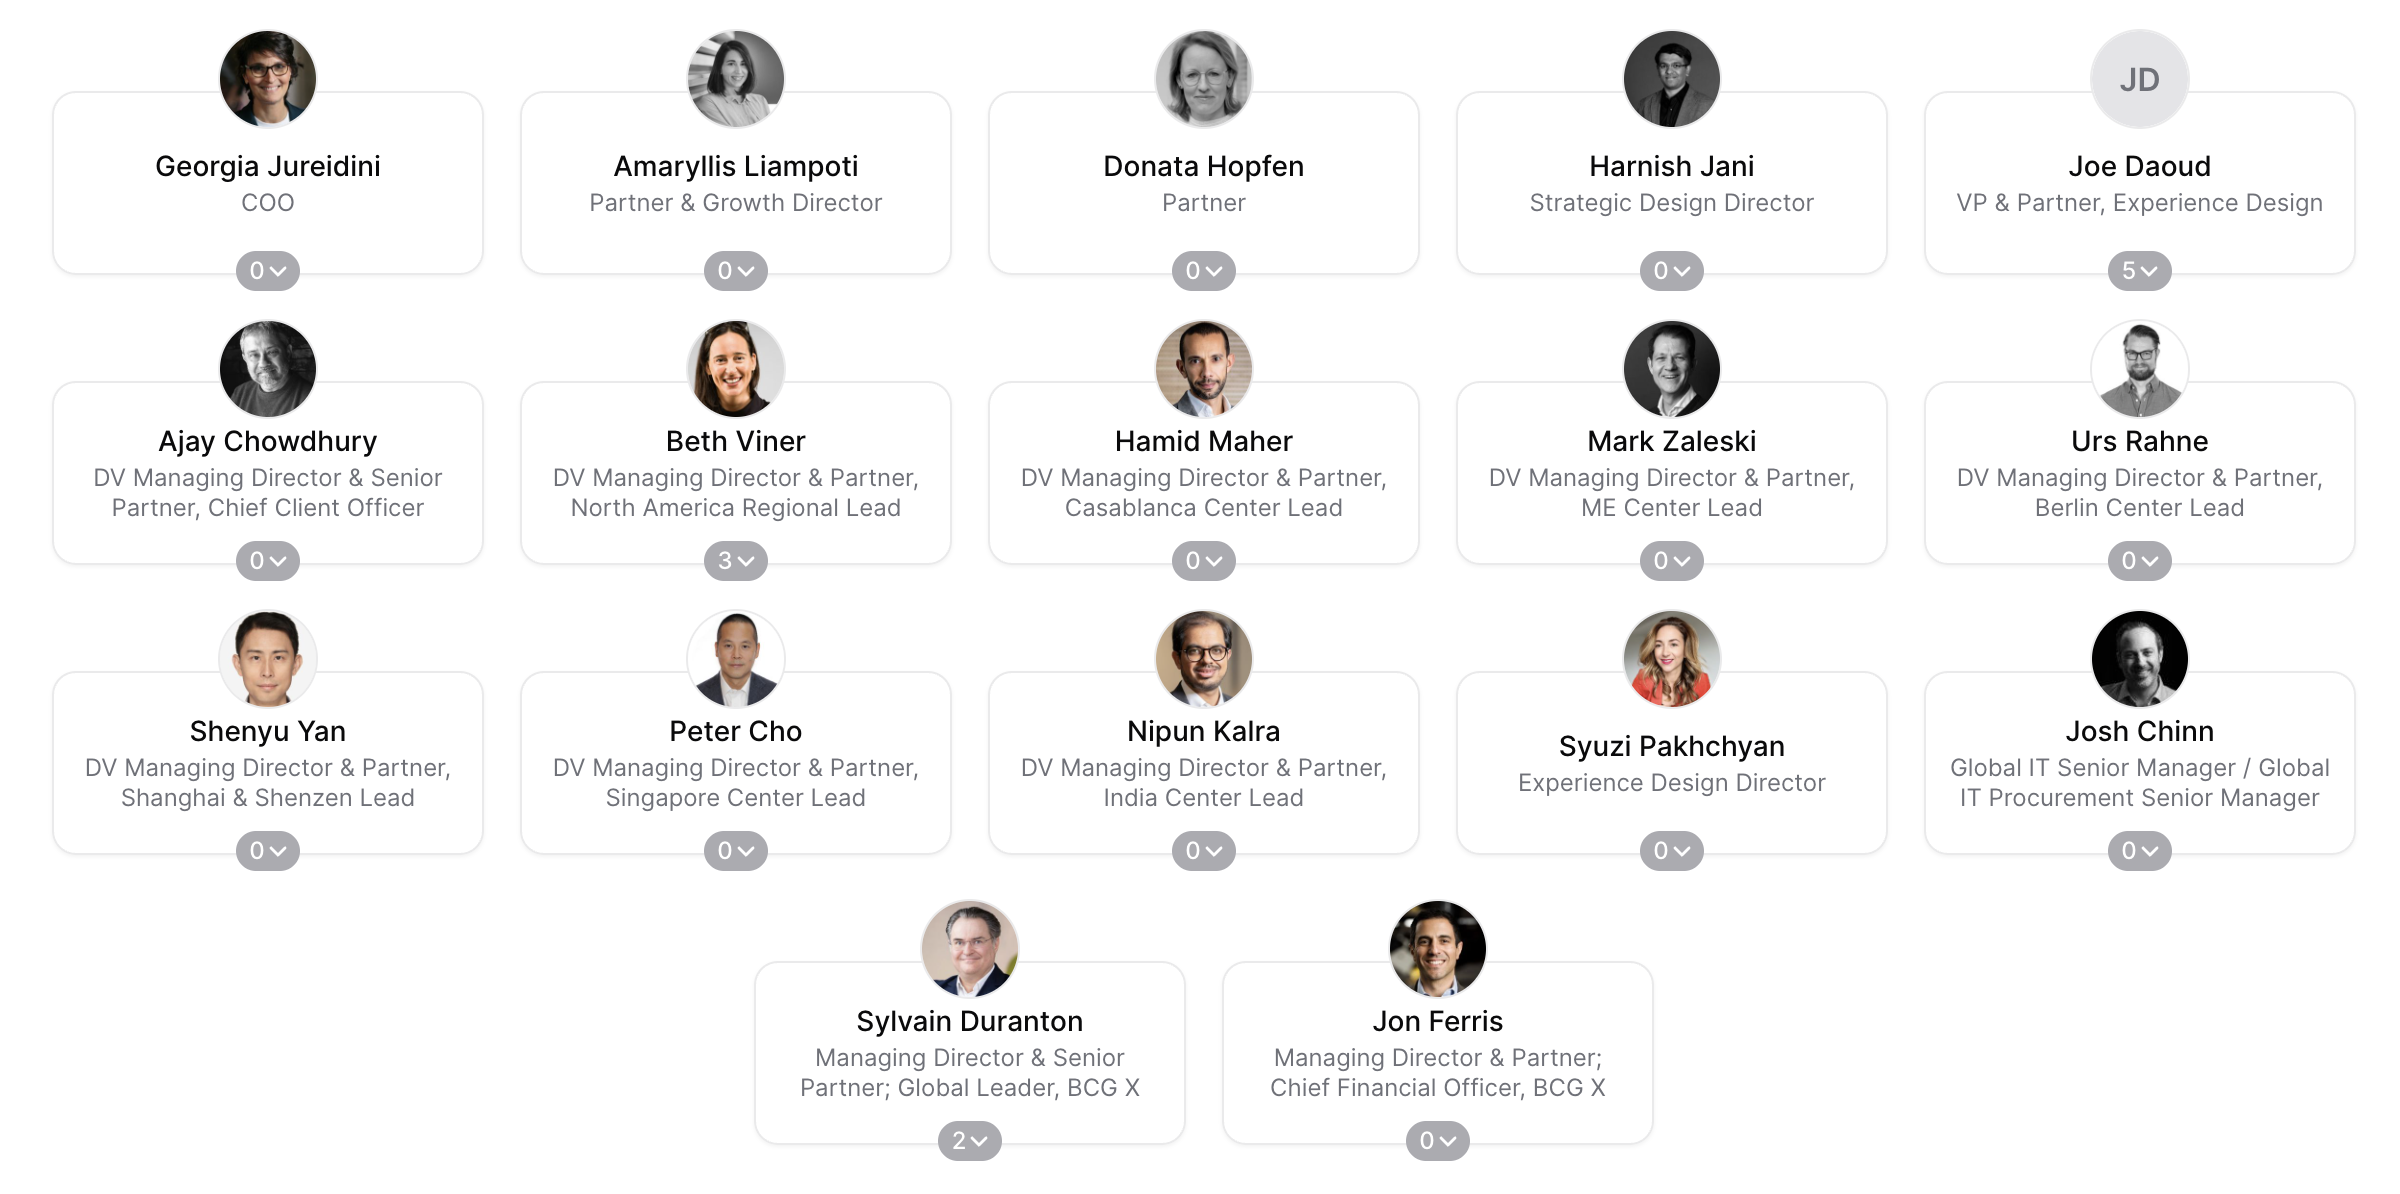
\includegraphics[width=\linewidth]{Images/Executive Leadership Board.png}
    \captionof{figure}{Executive Leadership Board}\cite{executive-leadership-board}
    \label{fig:executive}
\end{center}
\noindent
\mynewline
BCG X’s organizational design promotes effective decision-making, seamless collaboration across global teams, and responsiveness to client needs, leveraging both hierarchical and regional structures.

% Organizational Culture
\subsection{Organizational Culture}
BCG X fosters a dynamic organizational culture defined by innovation, inclusivity, and entrepreneurial spirit. Its culture encourages team members to embrace challenges, take risks, and collaborate openly to drive transformative solutions for clients.\mynewline

Key aspects of BCG X’s organizational culture include:
\begin{itemize}
    \item \textbf{Innovation and Entrepreneurship }\\
        Innovation is central to BCG X's culture, which consistently emphasizes entrepreneurial mindsets, encouraging individuals to explore new ideas, technologies, and methodologies. Employees are supported in developing digital solutions that significantly impact businesses and industries.
    \item \textbf{Inclusivity and Employee Well-being }\\
        BCG X prioritizes a culture of inclusivity and well-being, providing a supportive environment that values diverse perspectives and encourages personal and professional growth. The organization actively supports employees through wellness programs, career coaching, tuition reimbursement, and structured promotion pathways.
    \item \textbf{Open Communication and Collaboration }\\
        Transparent and open communication is encouraged within the organization, fostering a collaborative environment where ideas can flow freely. Employees are empowered to communicate openly, enabling swift decision-making and fostering strong internal relationships and teamwork.
    \item \textbf{Ambition and Growth Orientation }\\
        The organizational culture at BCG X highly values ambitious, growth-oriented individuals who are comfortable navigating ambiguity and pushing boundaries. This ambition is reflected in rapid innovation cycles, strategic client engagements, and a constant drive to achieve impactful outcomes.
\end{itemize}

Overall, BCG X’s organizational culture underpins its ability to deliver high-impact digital transformation and innovation, driven by motivated, collaborative, and empowered teams.


% Project Framework
\section{Project Framework}


% Agentic AI in Legal Operations
\subsection{Agentic AI in Legal Operations}
Agentic AI represents an innovative shift from traditional imperative systems toward autonomous decision-making processes in various business functions. It involves specialized AI agents that are designed to autonomously determine actions based on high-level goals, dynamically adapting to new data and operational conditions. In legal operations specifically, Agentic AI significantly improves flexibility, scalability, and efficiency by automating complex workflows traditionally reliant on extensive manual intervention.\mynewline

Agentic AI platforms in legal applications are equipped with capabilities such as automated clause selection, smart contract data mapping, continuous monitoring, and compliance verification. These autonomous capabilities streamline the traditionally manual processes involved in contract drafting, validation, and compliance monitoring, significantly reducing contract processing time and increasing accuracy.

%Digital Contract Management
\subsection{Digital Contract Management}
The process of contract management traditionally involves manual drafting, iterative feedback loops, and approval workflows that often lead to inefficiencies, errors, and delays. Digital Contract Management (DCM) solutions have emerged to address these issues, aiming to centralize, automate, and optimize the entire lifecycle of contract operations—from initial drafting to final execution and continuous monitoring.\mynewline

DCM employs sophisticated AI-driven agents capable of real-time collaboration, intelligent clause insertion, and automated verification. This approach enhances operational efficiency, reduces manual effort in repetitive tasks, and improves compliance by automatically tracking regulatory changes and adapting contracts accordingly. Digital contract management thus transforms legal operations into agile, scalable, and error-resistant processes, significantly boosting organizational productivity and risk management.

% Need for Intelligent Legal Workflow Systems
\subsection{Need for Intelligent Legal Workflow Systems}
Traditional legal workflows suffer from manual bottlenecks, fragmented processes, and compliance risks due to frequent internal and external regulatory changes. The manual approach limits scalability and visibility, causing significant inefficiencies in managing contractual obligations and deadlines.\mynewline

Implementing Intelligent Legal Workflow Systems, powered by Agentic AI, addresses these pain points by automating repetitive tasks, providing real-time monitoring of contract lifecycles, and offering predictive insights into compliance and risk management. These systems ensure seamless collaboration between various stakeholders, streamline approval processes, and mitigate risks through automated compliance checks. The result is a robust, scalable framework capable of handling complex legal workflows with improved transparency and accountability.

% Problematic
\subsection{Problematic}
Current contract management and legal operations rely heavily on manual inputs, iterative feedback loops, and scattered stakeholder communications, leading to inefficiencies, compliance risks, and delays. Contract drafting and validation processes are especially impacted, often resulting in lengthy negotiation cycles, limited visibility into contract deadlines, and difficulty in ensuring consistent regulatory compliance across different jurisdictions. The lack of automated systems further exacerbates these issues, causing increased operational costs and elevated risk profiles.

% Objectives
\subsection{Objectives}
This project aims to deploy and evaluate the effectiveness of an AI-driven intelligent contract management platform leveraging Agentic AI to transform traditional legal operations into streamlined, scalable, and automated processes.\mynewline

The specific objectives include:
\begin{itemize}
    \item Automating repetitive and manual contract drafting tasks through AI pre-filling and intelligent clause selection.
    \item Establishing real-time, AI-driven monitoring and compliance validation of contracts.
    \item Enhancing collaboration and efficiency across multiple stakeholders via automated workflows and digital signatures.
    \item Reducing overall contract processing time and manual effort significantly (40-60\% reduction target).
    \item Minimizing compliance risks through automated regulatory updates and monitoring, aiming for a 30\% risk reduction.
\end{itemize}

Achieving these goals will provide a standardized, scalable solution capable of significantly enhancing efficiency, compliance, and risk management across legal operations.

% Project Management
\section{Project Management}

% Progress Monitoring
\subsection{Progress Monitoring}
During my internship, we did not strictly adhere to an agile methodology. Instead, we implemented a weekly meeting schedule supplemented by urgent meetings for critical issues, such as troubleshooting problems or addressing pressing concerns. This approach ensured a consistent overview of project developments while allowing for the timely resolution of emergent needs. Additionally, I met one-on-one with my mentor weekly. These meetings allowed me to present the progress made, receive feedback, and discuss any open questions or issues. The feedback provided valuable insights from different perspectives and played a crucial role in refining the project’s functional requirements. Our sync-up meetings typically included status updates, demonstrations of functionality (if applicable), discussion of open questions or issues, and outlining next steps in the project.

% Collaboration Tools
\subsection{Collaboration Tools}
Using collaboration tools within a team offers several benefits. They play an important role in enhancing teamwork and communication within a team, enabling seamless communication through instant messaging and video conferencing. They also facilitate efficient collaboration on shared documents and projects, providing centralized repositories for knowledge sharing and documentation. Here is a list of collaboration tools used during my internship (\textit{Figure~\ref{fig:tools}}):
\begin{center}
    \centering
    
\includegraphics[width=\textwidth]{Images/tools.png}
    \captionof{figure}{Communication Tools}
    Logos from Outlook\cite{Outlook}, Slack\cite{slack}, and Zoom\cite{zoom}.
    \label{fig:tools}
\end{center}
\begin{itemize}
    \item \textbf{\textit{Slack}}: A well-liked platform that offers file transfers, instant messaging, and robust message searching. It integrates with numerous other tools, including Zoom and Outlook, offering interesting features to facilitate communication;
    \item \textbf{\textit{Zoom}}: A cloud-based video conferencing tool that simplifies the  hosting of virtual one-on-one or team meetings. This remote communication tool connects remote team members with one another, providing strong audio, video, and collaboration features;
    \item \textbf{\textit{Outlook}}: Serving as an email management platform, Outlook enables users to send and receive emails, manage calendars, store contact information, and track tasks effectively;
    \item \textbf{\textit{Confluence}}:
          \begin{center}
              \centering
              
\includegraphics[width=0.2\textwidth]{Images/confluence_logo.png}
              \captionof{figure}{Confluence Logo} \cite{Confluence}
              \label{fig:confluence}
          \end{center}
          A collaborative wiki-style platform developed by Atlassian, serving as a central knowledge base and documentation tool. It allows us to document projects comprehensively, ensuring ease of understanding.
\end{itemize}
\subsection{Internship Planning}
My internship was conducted into two phases: the onboarding phase and the project phase.
\subsubsection[Onboarding Phase]{Onboarding Phase}
The first phase was dedicated to onboarding, ensuring a smooth integration into the company and providing the necessary training before starting the project. This phase included several key activities:

\begin{itemize}
    \item \textbf{Account and Software Setup }\\
          The initial step involved setting up various accounts and software essential for daily operations, to ensure we had access to the necessary tools and platforms. This step included also familiarization with the company’s processes and workflows, including understanding the organizational structure and communication tools.
    \item \textbf{Generic Training }\\
          The training provided an excellent opportunity to expand our skills and knowledge in various areas of software development.
          The generic training provided access to Oracle’s learning resources and covered essential tools and platforms, including:
          \begin{itemize}
              \item Communication tools (Slack);
              \item Linux;
              \item Oracle Cloud Infrastructure (OCI);
              \item Developer tools (Git, Bitbucket, Jira);
              \item DevOps;
              \item Scripting;
              \item APEX.
          \end{itemize}
    \item \textbf{Specific Training }\\
          For my specific training, I focused on Oracle Linux and virtualization technologies, as these are essential for our team’s system testing and validation efforts. This training involved gaining more experience in working with Oracle Linux and mastering virtualization tools like QEMU and Libvirt.
\end{itemize}
\subsubsection[Project Phase]{Project Phase}
After the onboarding phase, the focus shifted to the project phase. The following Project Gantt Diagram (\textit{Figure~\ref{fig:gantt}}) illustrates the timeline and sequence of the project phases.

\begin{center}
    \centering
    
\includegraphics[width=\textwidth]{Images/Gantt Diagram.png}
    \captionof{figure}{Gantt Diagram}
    \label{fig:gantt}
\end{center}

\section{Conclusion}
This chapter provided the context of this project. We presented the host organization and discussed the general framework of the project, focusing on its context, problematic, and objectives. We also described  the methodology employed during the internship and the project's planning.